\subsection{Lavpasfilter}
For at teste, hvorvidt lavpasfilteret fungerer sammenlignet med de opstillede krav i \autoref{sec:lavpas_krav} visualiseres forskellen mellem det ufiltrede samt filtrede signal. 
De indsendte signaler er fra det optagede signal fra pilotforsøget. \autoref{sec:pilotforsoeg}. Disse sendes til mikrokontrollen via en UART-forbindelse, hvorved den retunerede værdi modtages. De indsendte samt returnerede værdier er visualiseret i MATLAB og fremgår af \autoref{fig:lavpas_imp}

\begin{figure}[H]
\centering
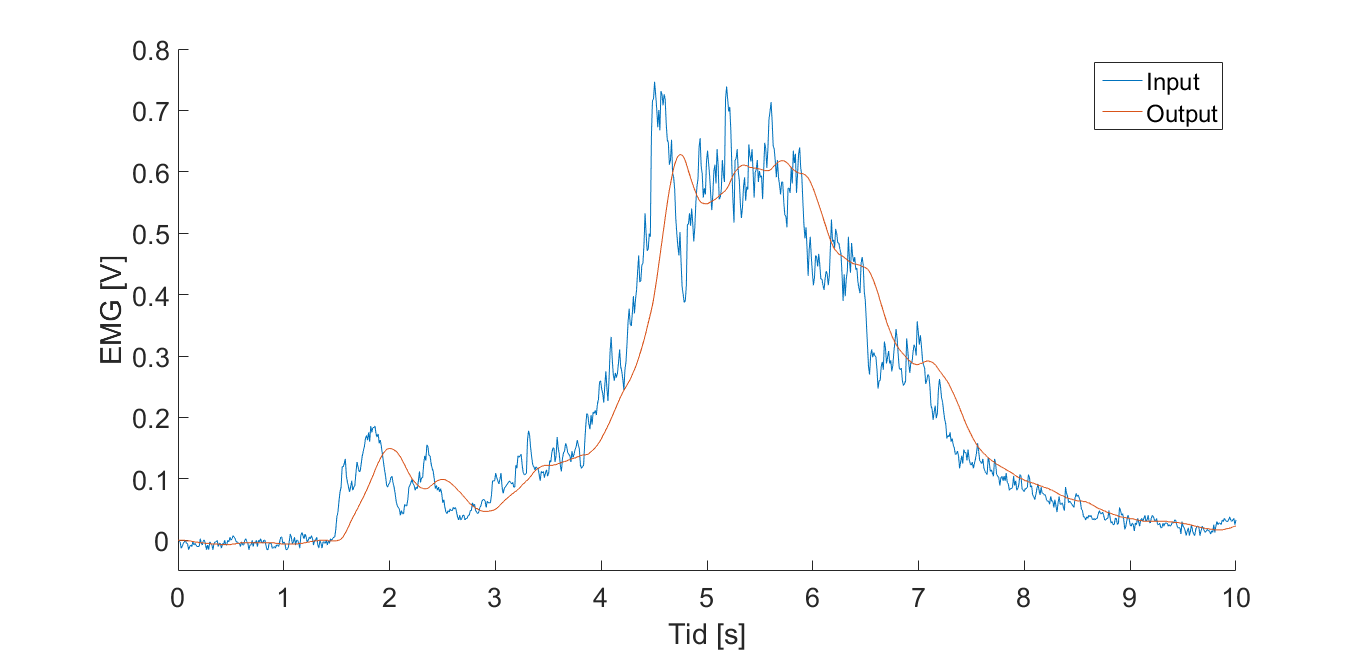
\includegraphics[width=0.8\textwidth]{figures/EMG_test}
\caption{Lavpasfilter programmeret i PSoC visualiseret i MATLAB}
\label{fig:lavpas_imp}
\end{figure}

Figuren illustrer, at inputsignalet følger det ufiltrede signal dog med et delay. Til måling af behandlingstiden af dette, programmeres en timer funktion i mikrokontrolleren, der retunerer behandlingstiden til MATLAB. Ud fra dette ses et delay på XX sekunder. Dette krav accepteres, da dette ikke vil få en betydning, da der optages et antal samples og på baggrund af flere samples vurderes det, hvorvidt muskelaktiviteten er stigende eller faldende, hvilket medvirker til at systemet udfører en naturlig bevægelse.


For at vurdere om filteret er dæmpende i forhold til de opstillede krav, udføres en sweep-test af frekvenser fra $0-15~Hz$ med en funktionsgenerator. Dette frekvensområde er valgt på baggrund af målinger fra \autoref{sec:pilotforsoeg}, hvor det fremgår, at signalet ligger mellem $0,4-10Hz$.  Da funktionsgeneratoren ikke kan indstilles til en frekvens på $0~Hz$ indstilles denne til $1 \mu~Hz$. Amplituden sættes til 1 $V_{pp}$ med et offset på $1.65~V$, som er det halve af spændingsforsyningen på $3,3~V$. Værdierne er ganget med $\frac{3,3V}{2048}$ for at omregne det til spænding. De $3,3~V$ svarer til spændingsforsyningen, mens de 2048 er svarede til ADC'ens arbejdsområde. Resultatet af sweeptesten fremgår af \autoref{fig:lavps_sweep} \textbf{a)}, mens \textbf{b)} viser kurven for $V_{pp}$ gennem swepp'et.

\begin{figure}[H]
\centering
\includegraphics[width=0.8\textwidth]{figures/Lavpass_test}
\caption{Lavpasfiltrering af sweeptest fra 0 til $15~Hz$. Målingen er foretaget med et inputsignal svarende til en sinusbølge med en peak-to-peak på $1~V$. Signalet samples med en frekvens på $100~Hz$. Figur \textbf{a} viser signalet efter filtrering, mens \textbf{b)} viser $V_{pp}$ gennem en sweeptest. Signalet er opdelt i vinduer af 500 milisekunders varighed og overlapper hinanden med 50 \%.}
\label{fig:lavps_sweep}
\end{figure}


En dæmpning på $-3~dB$ for den valgte knækfrekvens på $5~Hz$ bestemmes samt en decade længere ude svarende til en frekvens på $15~Hz$. Da der anvendes et 2. ordens filter, skal denne frekvens dæmpes ved $-40~dB$. Outputspændingen ved disse dæmpningsfaktorer er udregnet ved \autoref{equ:daempning1} og \autoref{equ:daempning2}. 

\begin{equation} \label{equ:daempning1}
-3~dB = 20 \cdot log_{10} \cdot (\frac{V_{out}}{0,1}) \Rightarrow V_{out} = 0,07 V
\end{equation}
\begin{equation} \label{equ:daempning2}
-40~dB = 20 \cdot log_{10} \cdot (\frac{V_{out}}{0,1}) \Rightarrow V_{out} = 0,01 V
\end{equation}

\noindent
Da målingerne for $V_{pp}$ er downsamplet er det ikke muligt at aflæse nøjagtige værdier, hvorfor der tages udgangspunkt i de nærmeste værdier. Værdierne for $5~Hz$ er $0,06~V$, mens det for $15~Hz$ er $0,008~V$. Afvigelsen fremgår af \autoref{equ:afvigelse1} og \autoref{equ:afvigelse2}.


\begin{equation} \label{equ:afvigelse1}
Afviglese_{5~Hz} = \frac{0,06V-0,07V}{0,07V} = -0,14  = - 14%
\end{equation}
\begin{equation} \label{equ:afvigelse2}
Afvigelse_{15~Hz} = \frac{0,008V-0,01V}{0,01V} = -0,20  = -20%
\end{equation}

\noindent 
Afvigelserne er for $5~HZ$ 14\%, mens det for $15~Hz$ er 20\%. Dette betyder at filteret ikke dæmper signalet nok. Da målingerne for outputspændingen, målt ved de forskellige frekvenser, ikke er målt nøjagtig grundet downsampling, er det forventet, at der er en større afvigelse fra den teoretiske udrening. På baggrund af dette godtages filteret. 
